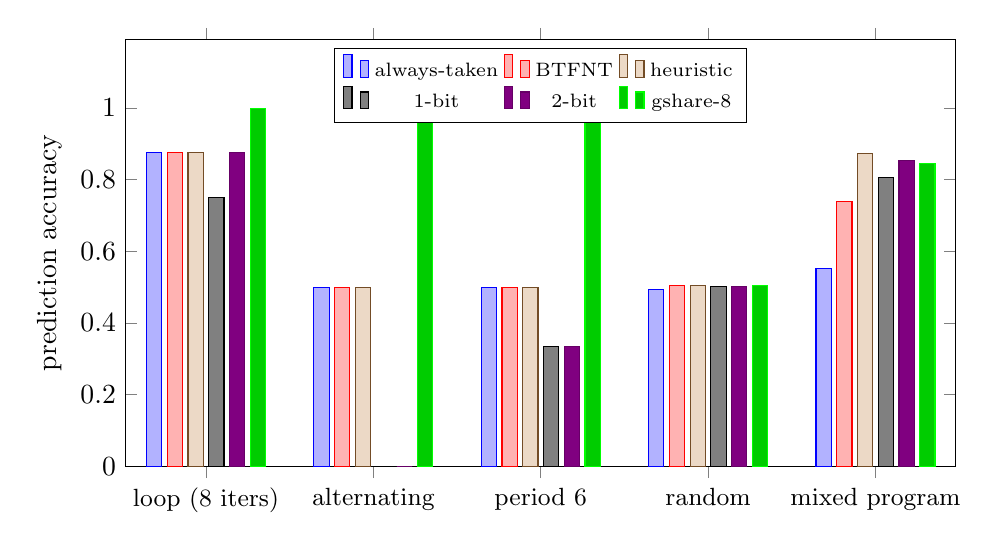
\begin{tikzpicture}
\begin{axis}[ybar, width=\textwidth, height=7cm, bar width=5.5pt, ymin=0, ymax=1.19, ylabel={prediction accuracy},
  symbolic x coords={loop (8 iters),alternating,period 6,random,mixed program}, xtick=data, x tick label style={font=\small},
  legend style={font=\scriptsize, at={(0.5,0.98)}, anchor=north, legend columns=3}, enlarge x limits=0.12]
\addplot coordinates {(loop (8 iters),0.8750) (alternating,0.5000) (period 6,0.5000) (random,0.4945) (mixed program,0.5527)};
\addlegendentry{always-taken}
\addplot coordinates {(loop (8 iters),0.8750) (alternating,0.5000) (period 6,0.5000) (random,0.5055) (mixed program,0.7391)};
\addlegendentry{BTFNT}
\addplot coordinates {(loop (8 iters),0.8750) (alternating,0.5000) (period 6,0.5000) (random,0.5055) (mixed program,0.8725)};
\addlegendentry{heuristic}
\addplot coordinates {(loop (8 iters),0.7505) (alternating,0.0000) (period 6,0.3334) (random,0.5017) (mixed program,0.8054)};
\addlegendentry{1-bit}
\addplot coordinates {(loop (8 iters),0.8750) (alternating,0.0000) (period 6,0.3334) (random,0.5028) (mixed program,0.8530)};
\addlegendentry{2-bit}
\addplot coordinates {(loop (8 iters),0.9995) (alternating,0.9994) (period 6,0.9995) (random,0.5036) (mixed program,0.8439)};
\addlegendentry{gshare-8}
\end{axis}
\end{tikzpicture}